% THIS IS SIGPROC-SP.TEX - VERSION 3.1
% WORKS WITH V3.2SP OF ACM_PROC_ARTICLE-SP.CLS
% APRIL 2009
%
% It is an example file showing how to use the 'acm_proc_article-sp.cls' V3.2SP
% LaTeX2e document class file for Conference Proceedings submissions.
% ----------------------------------------------------------------------------------------------------------------
% This .tex file (and associated .cls V3.2SP) *DOES NOT* produce:
%       1) The Permission Statement
%       2) The Conference (location) Info information
%       3) The Copyright Line with ACM data
%       4) Page numbering
% ---------------------------------------------------------------------------------------------------------------
% It is an example which *does* use the .bib file (from which the .bbl file
% is produced).
% REMEMBER HOWEVER: After having produced the .bbl file,
% and prior to final submission,
% you need to 'insert'  your .bbl file into your source .tex file so as to provide
% ONE 'self-contained' source file.
%
% Questions regarding SIGS should be sent to
% Adrienne Griscti ---> griscti@acm.org
%
% Questions/suggestions regarding the guidelines, .tex and .cls files, etc. to
% Gerald Murray ---> murray@hq.acm.org
%
% For tracking purposes - this is V3.1SP - APRIL 2009

\PassOptionsToPackage{pdfpagelabels=false}{hyperref}
\setlength{\paperheight}{11in}
\setlength{\paperwidth}{8.5in}
\documentclass{acm_proc_article-sp}
\usepackage{hyperref}
\usepackage{url}
\usepackage{mdwlist}
\usepackage{enumitem}
\setitemize{noitemsep,topsep=0pt,parsep=0pt,partopsep=0pt}

% This gives LaTeX permission to insert extra line breaks instead of
% trying to fit too much in a single line. This helps with the
% "Overfull \hbox" warnings (but so far doesn't eliminate all of them)
\pretolerance=2500

% This inserts an ugly black box next to blatant violations of the 
% overfull hbox rule
\overfullrule=2cm

% Remove the blank space for copyright; see http://www.acm.org/sigs/publications/sigfaq#a21
\makeatletter
\let\@copyrightspace\relax
\makeatother

\begin{document}

\title{Spring XD: A Modular Distributed Stream and Batch Processing System}

% You need the command \numberofauthors to handle the 'placement
% and alignment' of the authors beneath the title.
%
% For aesthetic reasons, we recommend 'three authors at a time'
% i.e. three 'name/affiliation blocks' be placed beneath the title.
%
% NOTE: You are NOT restricted in how many 'rows' of
% "name/affiliations" may appear. We just ask that you restrict
% the number of 'columns' to three.
%
% Because of the available 'opening page real-estate'
% we ask you to refrain from putting more than six authors
% (two rows with three columns) beneath the article title.
% More than six makes the first-page appear very cluttered indeed.
%
% Use the \alignauthor commands to handle the names
% and affiliations for an 'aesthetic maximum' of six authors.
% Add names, affiliations, addresses for
% the seventh etc. author(s) as the argument for the
% \additionalauthors command.
% These 'additional authors' will be output/set for you
% without further effort on your part as the last section in
% the body of your article BEFORE References or any Appendices.

\numberofauthors{5} %  in this sample file, there are a *total*
% of EIGHT authors. SIX appear on the 'first-page' (for formatting
% reasons) and the remaining two appear in the \additionalauthors section.
%
\author{
% You can go ahead and credit any number of authors here,
% e.g. one 'row of three' or two rows (consisting of one row of three
% and a second row of one, two or three).
%
% The command \alignauthor (no curly braces needed) should
% precede each author name, affiliation/snail-mail address and
% e-mail address. Additionally, tag each line of
% affiliation/address with \affaddr, and tag the
% e-mail address with \email.
%
% 1st. author
\alignauthor Sabby Anandan
% 2nd. author
\alignauthor Marius Bogoevici
% 3rd. author
\alignauthor Glenn Renfro
\and  % use '\and' if you need 'another row' of author names
% 4th. author
\alignauthor Ilayaperumal Gopinathan
% 5th. author
\alignauthor Patrick Peralta
}
% There's nothing stopping you putting the seventh, eighth, etc.
% author on the opening page (as the 'third row') but we ask,
% for aesthetic reasons that you place these 'additional authors'
% in the \additional authors block, viz.

% Just remember to make sure that the TOTAL number of authors
% is the number that will appear on the first page PLUS the
% number that will appear in the \additionalauthors section.

\maketitle
\begin{abstract}
Spring XD is a unified, distributed and extensible system for data ingestion,
real time analytics, batch processing, and data export. The objective of
Spring XD is to simplify the development and deployment of streaming and batching
data applications. Spring XD is a Java based Apache 2 licensed open source project developed
by Pivotal\cite{pivotal}.  This paper discusses the motivation, architecture, and use cases
for Spring XD.
\end{abstract}

\section{Introduction}

The era of Big Data has introduced many new technologies for data storage
and processing. The success and high demand for horizontally scalable
solutions such as HDFS, Spark, and Kafka demonstrates this need. At the
same time, enterprises have invested heavily in older and proven
technologies such as SQL databases and messaging systems. For enterprises
to adopt the emerging technologies, there must be a way to easily
connect with existing systems.

Since its inception in 2004, the main objective of the Spring Framework
has been to simplify application development. At the time, Java developers
were struggling with EJBs, boilerplate JDBC, and JMS. Today's developers
are dealing with an explosion of data and the leading-edge tools to
manage and process this data.

Expanding upon the success of existing technologies in the Spring portfolio
such as Spring Integration and Spring Batch, Spring XD provides a runtime
environment that integrates with a plethora of technologies, both established
and up-and-coming.

Although enterprise system integration is one of the strengths of Spring XD,
it is a compelling technology for brand new applications that have streaming
or batch data processing requirements. Spring XD features a built in
interactive shell for creating streams or jobs without writing any Java code.
This allows for quick development cycles and easy experimentation.

Creating a stream in Spring XD is a simple concept for those familiar with
UNIX streams and pipes. Consider the following shell command:

\verb;tail -f /tmp/log.txt | grep ERROR;

The tail command will continuously display the file contents. The |
will pipe the output of tail to grep, which will filter out all
lines that do not contain the string ERROR.

The equivalent using Spring XD looks like this:

\verb;stream create -name error-filter -definition;\\*
\verb;  "tail -name=/tmp/log.txt | filter;\\*
\verb;  --expression=payload.contains('ERROR') | log";

While this specific example will only tail a local file, a distributed 
ingestion stream that aggregates, filters, and stores log file analytics
can just as easily be created with Spring XD.


\section{Architecture}
This section describes the internal architecture of Spring XD. See figure~\ref{fig:architecture}.

\subsection{Application Context}
The foundation of Spring XD is the Spring application context. The application context is a dependency injection framework that is used to instantiate objects along with their dependencies \cite{spring-framework-reference}. 

\subsection{Modules}


\begin{figure}[ht]
\centering
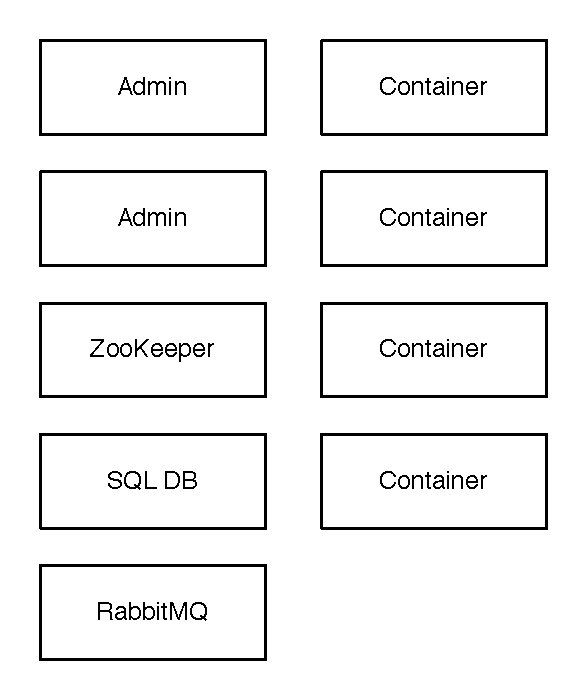
\epsfig{file=XD-sample.eps, height=2in, width=2in}
\caption{Spring XD Architecture.}
\label{fig:architecture}
\end{figure}

Here is where we get into the fine grained details.

\section{Modules}
\label{sec:Modules}
A Spring XD Module \cite{modules} is a data processing unit and as mentioned above
there are four types: source, processor, sink, and job. Modules in Spring XD are defined 
in their own application context. This allows for easy encapsulation and life cycle 
management for modules. Additionally, the use of an application context allows for easy 
module expansion.  Spring XD uses Spring Integration \cite{spring-integration-reference} 
as its foundation for implementing modules. A module is comprised of component that
implements the data processing logic and one or more connectors(known as channels)
that connect to the underlying message bus.

\par

Spring XD offers a suite of 23 sources, 24 sinks, 9 processors and 9 jobs that are ready 
to use at startup.  These modules integrate with a variety of well known and popular
data stores and processing systems such as JDBC, HDFS, MongoDB, Spark, Kafka, RabbitMQ,
Sqoop etc.,  If an existing module does not meet the needs of a given use case, Spring XD
supports developing custom modules.

Spring XD sink and source modules are Message Endpoints 
\cite{enterprise-integration-pattern-message-endpoint} 
that are responsible for sending data to and receiving data from external applications
respectively. A source is the entry point for data into the stream. A sink is the module that dispatches
the stream's results to an external application or storage system. A Processor
module is used to modify data transmitted from the source to sink. Multiple processors may be chained together.
Batch jobs are used to execute batch processing steps on a set of data.

\par

\subsection{Source}
Source modules receive inbound data and send to downstream modules in the stream or to a batch job
which could be triggered with the data. There are two source types: poller and event driven.
A poller source is based on the polling consumer pattern \cite{enterprise-integration-pattern-pollingconsumer}.
It polls an external application (such as a web service, FTP server, database) for data at a
configurable interval. An event driven source is based on the event driven
consumer pattern \cite{enterprise-integration-pattern-eventdrivenconsumer} which
opens a port to listen for incoming data that is pushed from an external application.

\par

In the case of a source module there is an ``output'' connector channel to dispatch data
transmitted by the module to a downstream module(see figure~\ref{fig:sourcembc}.)

\par

\begin{figure}[ht]
\centering
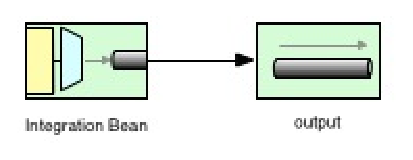
\epsfig{file=integration-module-output-channel.eps, height=.6in, width=1.75in}
\caption{Source Module Basic Components}
\label{fig:sourcembc}
\end{figure}

\par

\subsection{Processor}
A processor is the module that receives data from a source or a previous processor
module's output and performs the transformation operation and sends the data
into a sink module or a downstream processor module. The basic processor is
comprised of both an ``input'' and an ``output'' connector channels and the data processing component.
The input channel receives all data from the upstream module and dispatches them to
the data processing component(see figure~\ref{fig:processormbc}.) It is the responsibility of
this component to transform the data. The transformed data is then sent to the downstream module
via the output channel.

\par

\begin{figure}
\centering
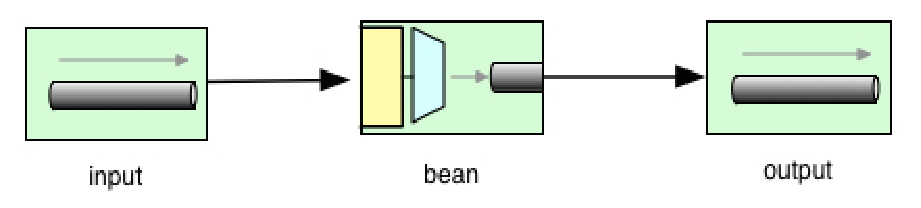
\epsfig{file=module-processor.eps, height=.6in, width=2.5in}
\caption{Processor Module Basic Components}
\label{fig:processormbc}
\end{figure}

\par

\subsection{Sink}
Sink modules convert and deliver data out of the stream in a format consumable by
an external application.  There are two types of sinks: analytic and delegate.
An analytic sink is used to perform analytic operations such as count, gauge on the
incoming data and store the result into metric repository(See section~\ref{sec:Analytics}.)
A delegate sink translates data to the format expected by the external application.
After transforming the data, the resulting data is sent to the external application.

\par

The basic sink is comprised of a ``input'' channel connector and a data processing
component. The input channel receives data from the stream and dispatches
messages to the bean (see figure~\ref{fig:sinkmbc}.) The sinks
included in Spring XD have configurable options for retries in case of failure.

\par

\begin{figure}
\centering
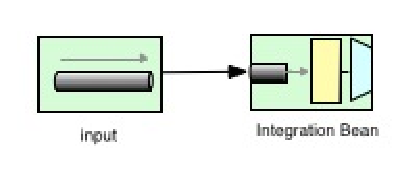
\epsfig{file=integration-module-input-channel.eps, height=.6in, width=1.75in}
\caption{Sink Module Basic Components}
\label{fig:sinkmbc}
\end{figure}

\par

\subsection{Job}
Spring XD uses Spring Batch \cite{spring-batch-reference}, a JSR standardization (JSR-352)
of batch workload data processing as the foundation for implementing
job modules. A job enables users to execute enterprise batch processes within Spring XD.
Jobs are typically used when running long lasting tasks that have transactional requirements.
To account for failure scenarios, the workflow in the job can be designed to restart and 
resume operation or roll-back the transaction altogether. A job can be triggered by the
stream with the data that act as the input to start the batch processing. This makes
streams and job modules unified under a single platform.

\par

A job is typically comprised of a job definition along with the supporting
data processing components as shown in figure~\ref{fig:batchmbc}.
In some cases the job definition alone is sufficient to implement the desired behavior.

\par

\begin{figure}
\centering
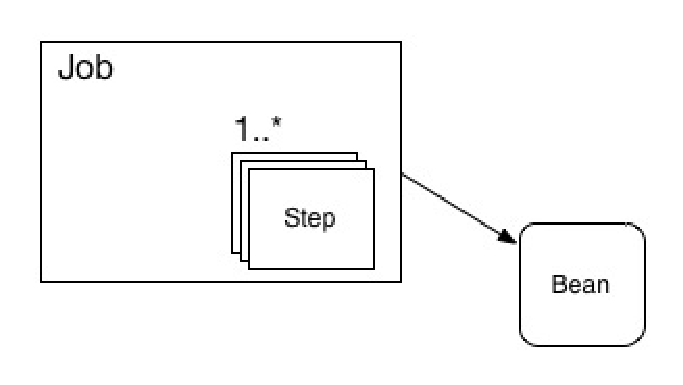
\epsfig{file=integration-batch.eps, height=.8in, width=2in}
\caption{Batch Basic Components}
\label{fig:batchmbc}
\end{figure}

\par 

\subsection{Composite}
A Composite module provides a way to create a single module comprised of
multiple modules (processing chain) together.  A composite module can be used to prevent
duplication when a processing chain of modules is used frequently.
Performance is another reason to use composite modules, because messages between the 
modules that comprise the composite module will be transmitted in memory vs. the message 
bus.  

\par

\subsection{Module Registry}
Module Registry is the place where Spring XD looks for the modules for
deployment. A module can be bundled as an archive or defined along with its
dependencies inside the module registry. The modules are defined in
the modules directory and are segregated in subdirectories by
type: \texttt{modules/source}, \texttt{modules/processor},
\texttt{modules/sink} and \texttt{modules/job}. The module registry is
configurable and one can upload the modules to module registry via REST request.
During the deployment of the module, Spring XD runtime will load the modules
dynamically from the module registry.


\section{Analytics}

Spring XD provides support to perform data analytics by adding analytical operations into 
an XD module. While the main stream collects the data from various sources into big data 
store such as HDFS , the main stream can be tapped at various stages and the tapped data 
can further be analyzed. This capability lets the analysts to perform data analytics in a
non-invasive manner. The analytics module can also be implemented to write the analytics 
data result into a data store (sink module) or sending the results to subsequent modules 
for processing (processor module). 

\par

Spring XD has out of the box analytics modules such as counter, field value counter, 
aggregate counter, gauge, rich gauge. Spring XD provides support for running predictive 
analytics using PMML model scoring. There is a support to run a module that executes s
hell command. This helps running R or python based processor or sink module implementation
 which could perform dynamic model scoring easier. One can also run Spark MLLib job as a 
 XD job and get out of the box capability to monitor and manage the job.

\subsection {Basic Analytics}

To perform some of the basic analytic operations, Spring XD provides following out of the 
box modules. Since these modules are implemented to write the analytic results back to a
data store they are considered as XD sink modules. Writing the analytic data into a data 
store is implemented using an extensible data store repository implementation 
(currently in-memory and Redis). The written analytic data are exposed via REST API. 
This way one can write a simple end-to-end application quickly to gain access to the 
analytic data results.

\subsubsection {Counter}

This module counts the number of events triggered on various stages of a stream. 
The main stream can be tapped at various stages and one can count the number of 
messages sent out at each stage. The counter value gets written to the data store.
 
\subsubsection {Field Value Counter} 

When there is a need to count the occurrence of a specific field from the message 
payload at various stages of a stream, field value counter can be used. Out of the box, 
XD supports the following message payload types:
POJO (Java Bean), Tuple, JSON string

\subsubsection {Aggregate Counter}

Aggregate counter is similar to the simple counter but also keeps track of time period. 
One can query the total count values for each minute, hour, day and month of the period in 
which data was collected/analyzed. 

\subsubsection {Gauge}
Gauge is a metric that represents a single long value associated with a unique name. 
In Spring XD, the gauge metric sink expects a numeric value as a payload.

\subsubsection {Rich Gauge}
Rich Gauge is a metric that holds a double value associated with a unique name. In 
addition to the value, this metric keeps a running average along with the minimum and 
maximum values and the count.

\subsection {Predictive Analytics using PMML}

\subsection {Shell based processor/sink implementation}

\subsection{Spark MLLib}



\section {Monitoring and Management}
Spring XD provides multiple options for management and monitoring of
its runtime components, including the following:\begin{itemize*}
	\item admin servers
	\item container servers
	\item stream and job modules
\end{itemize*}

\subsection {Monitoring via JMX and HTTP}
The runtime health, environment, and metrics information for these components
may be accessed via REST endpoints exposed by Spring Boot\cite{spring-boot}.
This functionality is also exposed via JMX; thus JMX clients such as JConsole
and Jolokia are supported.

\subsection {Management GUI}
Spring XD comes with an administrative web UI which allows users to manage
and monitor the system. The UI allows for the deployment and un-deployment
of streams and batch jobs. Batch Job module creation, control (start/stop)
and exploring job/step execution details are also supported.

\subsection {Shell Interface}
Spring XD includes an interactive shell which connects to the admin server
via the REST API. The shell exposes all of the management functionality
of the admin server.



\section{Deployment}
This section describes deployment architectures with Spring XD.
\subsection{Lambda architecture}

The Lambda Architecture, introduced by Nathan Marz \cite{lambda-architecture-paper} is a generic, scalable and fault tolerant data processing archictecture. It attempts to provide a comprehensive solution to the problem of processing an extremely large set of data.


The Lambda Architecture has the following components:

\begin{itemize*}
\item A \emph{master dataset} comprising of all data known to the system, ideally in its rawest form;
\item A \emph{serving} or \emph{view layer} that provides the latest, most up-to-date view of the processed data, available for low-latency, ad-hoc querying;
\item A \emph{batch layer} that performs computationally intense calculations that and prepares the \emph{batch views} displayed by the \emph{serving layer};
\item A \emph{speed layer} that performs calculations on recent data only, its output combined with the \emph{batch views} by the \emph{serving layer}.
\end{itemize*}

The guiding principle of the Lambda architecture is an attempt to combine the high throughput of batch operations with the low latency of real-time computations. Each on its own, has its strenghts and weakness. While the highest throughput for computing large datasets is attained by relying on batch computations, the latter have the disadvantage of higher latency. Meanwhile, real-time computations may operate with low latency and produce results based on latest data quickly, but can't really handle the large amounts of data that batch processing can deal with. So, instead of relying on a single paradigm, the lambda architecture employs both, allowing them to complement each other.

A detailed view of the Lambda Architecture can be viewed in figure [TBD]

\subsubsection {Master dataset in Spring XD}

While Spring XD does not provide a storage mechanism of its own, it integrates with a variety of data sources, allowing both reading (through its source[reference tbd, provide example] components), as well as writing, through its sink[reference tbd, provide examples] components. As such, it provides all the necessary means for ingesting data into a master dataset, also allowing for consolidating data from a variety of sources. 

TBD: provide an example of a simple stream

TBD: provide example of multiple streams with a namd queue sink and a stream with a named queue source. By sharing the sink, we create the master dataset out of multiple sources.

\subsubsection {Speed layer in Spring XD}

The Speed layer in Spring XD is handled by the streams. Transformers. Illustrate transformation of data, aggregation via counters.  

\subsubsection {Batch layer in Spring XD}

Jobs.

\subsubsection {Combining the two}

Stream-driven batch jobs. Taps. 

\subsubsection {View layer in Spring XD}

Externalized via sinks, output of batch jobs. Microservice architecture Example of a web application reading data off a set of tables written on by Spring XD. 

\subsubsection {Critique of the Lambda Architecture and Spring XD}

An often raised objection to the LA is the duplication of work (Quote Jay Kreps) that occurs during processing. More specifically, the necessity of writing the same processing code twice: once for the speed and once for the batch layer. However, due to the nature of Spring XD, the same business code can be shared between the two layers. This objection does not apply!


\subsection {Reactive architectures}

\subsection {Cloud deployment - does this even belong here??}


\section{Use Cases}
Few Fortune 100 and several Fortune 1000 companies are using Spring XD but all are under NDA. Following are some of the common use-cases that we have been supporting in the field.

\begin{itemize*}
\item \textbf{Fault Detection}: Spring XD connects machine data with enterprise infrastructure, middleware, and backend services. Continuous streams can be orchestrated in Spring XD to connect with various devices (i.e., machines). Consume and transform data of varied formats, analyze, predict failures, generate reports, and dispatch maintenance personnel - all in real-time.
\item \textbf{Enterprise Modernization}: Enterprises invest heavily on IT infrastructure, as the data resides at several layers in the enterprise architecture. Tight coupling with various products further adds more overhead with data management. Spring XD, as one-stop runtime, provides data integration adapters to consume data of varied formats (i.e., structures, unstructured, binary, ..) that reside in different toolchains (i.e., database, middlewares, in-memory grids, ..). Given the unified approach, enterprises' are equipped with developer-friendly fixtures to create pipelines using Spring XD. Pipelines connecting varied data producing and consuming agents eliminates the necessity of toolchains, maintenance overhead, or production support - Spring XD simplifies data collection and aggregation.
\item \textbf{Data Ingest}: Spring XD is a standard tool for ingesting data into Hadoop. Whether it is real-time (i.e., online) or batch (i.e., offline), you've fixtures to operationalize pipeline that fits your business needs.
\item \textbf{24/7 Production Pipelines}: The business demands highly available data streams with guaranteed data processing, to react in real-time accurately. Spring XD's runtime is highly reliable that can recover from failures seamlessly. Production running pipelines are long running tasks - there's no end. For ad-hoc operations such as querying, machine learning, or data crunching, `taps' in Spring XD are commonly adopted to fork the data from primary pipeline. This results in no disruption with the primary pipeline, at the same time ad-hoc demands can be fulfilled. 
\item \textbf{Closed-loop Analytics}: Spring XD orchestrates the entire analytics loop - gathering data from any source, triggering actions, handling feedback loops from machine learning models, and computing real-time predictions.
\item \textbf{Hadoop and Beyond}: Enterprises with existing investment in Hadoop technologies find Spring XD as one-stop orchestration platform. Whether it is MapReduce, Hive, Pig, or HBase scripts - developer experience is the same.
\end{itemize*}


\section{Related Work}
This section compares and contrasts Spring XD to similar projects.

\subsection{Spring XD and Spark}
Spark\cite{spark} is a general-purpose framework for large scale data processing.
In comparison with Hadoop's disk based MapReduce programming model, Spark's 
in-memory primitives provide immediate performance improvements.

The following features differentiate Spring XD and Spark Streaming.

\begin{itemize*}
\item Readily available integration adapters for data movements from various 
data sources in to Hadoop and others.
\item Ability to microbatch based on event count via Reactor and RxJava APIs.
\item Ability to create data pipelines to process one event at a time.
\item Flexibility to specify hosts to dictate the location of data computations.
\end{itemize*}

The following features differentiate Spring XD and Spark Batch processing.

\begin{itemize*}
\item Provides REST-API and lifecycle management for Spark jobs.
\item Extensible to integrate with other Batch systems.
\end{itemize*}

Recognizing the strengths of distributed data computations with Spark, Spring XD 
supports integration with Spark applications such as Spark Streaming, MLLib, and 
SparkSQL. Users familiar with Spark may implement the computation logic using 
Spark APIs in Java or Scala, and leave the orchestration to Spring XD. 
Spring XD also adds value by restarting the Spark Streaming driver to recover 
from fault scenarios.

\subsection{Spring XD and Storm}
Apache Storm\cite{storm} is a distributed computation system for real time stream 
processing.

The following features differentiate Spring XD and Storm.

\begin{itemize*}
\item Spring XD provides interactive Shell as opposed to Storm's API model to
create data pipelines.
\item Use of `taps' in Spring XD to build stream pipelines in isolation
without having to disrupt existing pipelines.
\item Loosely coupled `modules' in Spring XD are responsible for ingestion, analytics, 
data processing, machine learning or data export. Modules can be individually managed 
and dynamically scaled.
\item The notion of `composite modules' (unit\-of\-work) and colocation 
capabilities to fine-tune performance characteristics. 
\item Building upon the functional stream processing model, users have the option 
to choose from Reactor\cite{reactor}, Spark Streaming or RxJava APIs, to build 
complex data centric applications.
\end{itemize*}

Storm and Spring XD supports many common data sources and middleware's. 
For example, you can read and write data payloads from Apache Kafka topics both 
in Storm and Spring XD. Bolts/Spouts in Storm is analogous to Source/Processor/Sink 
in Spring XD. As stream processing frameworks, Storm and Spring XD can be used for 
similar use-cases.

\subsection{Spring XD and Flume}
Apache Flume\cite{flume} is a distributed system for collecting, aggregating and 
moving large data sets. 

The following features differentiate Spring XD and Flume.

\begin{itemize*}
\item High-level DSL to build streams and jobs.
\item Ability to monitor data workflows either via DSL, Admin UI, or custom 
dashboards.
\item Administer data pipelines through Admin UI.
\item Granular controls to manifest batch job and step execution to create 
complex data driven workflows.
\item Flexibility through `Deployment Manifest' to declaratively configure data 
partitioning strategy to route data to a specific consumer instance in the cluster.
\end{itemize*}

Flume offers HBase, Solr, and ElasticSearch sinks along with encryption support 
for Avro sources, which we are planning to address in our future releases.

\subsection{Spring XD and Oozie}
Oozie\cite{oozie} is a workflow scheduler engine to manage Hadoop \cite{hadoop} 
workloads such as MapReduce or Pig jobs. 

The following features differentiate Spring XD and Oozie.

\begin{itemize*}
\item Building upon Spring Batch, a JSR standardization (JSR-352) of batch 
workload data processing, Spring XD inherits workflow scheduling and execution 
functionaliites.
\item Provides out of the box batch jobs such as file-to-jdbc, file-to-hdfs, 
ftp-to-hdfs, hdfs-to-jdbc, hdfs-to-mongo, jdbc-to-hdfs, spark-job, and sqoop-job.
\item Ability to scale jobs without having to bring down the runtime.
\item Provides bidirectionality between real-time streaming and batch 
workflows to accommodate complex data processing use cases.
\item Ability to create and launch workflow-jobs from Admin UI. 
\item Ability to view historical snapshots of job executions from Admin UI.
\end{itemize*}

Oozie offers HCatalog integration, which we are planning to address in our 
future releases.

\subsection{Spring XD and Sqoop}
Apache Sqoop\cite{sqoop} assists with data transmission between Hadoop and relational 
databases.

The following features differentiate Spring XD and Sqoop.

\begin{itemize*}
\item Ability to orchestrate Pig, Hive, HBase, MapReduce or other batch systems.
\item Flexibility to extend batch workflow infrastructure to write custom tasklets.
\item High level configuration DSL to create, deploy and destroy batch workflows.
\item Flexibility to operationalize custom data pipelines through REST-APIs.
\item Unified functional programming support to build reactive-style data pipelines.
\end{itemize*}

Sqoop offers data validation, data merge, incremental data imports, and HCatalog 
integration among others. Recognizing the importance of these enterprise features, 
Spring XD provides an out of the box Sqoop job to take advantage and orchestrate 
data movements.

\section{Conclusion}

Mission critical data applications cannot live in a vacuum. The abundance of data
and specialized applications to process and store it require a holistic approach.
Spring XD is a formidable solution for managing the data flow and processing
between these applications. Spring XD integrates with systems ranging from decades
old RDBMS to cutting edge Big Data. The suite of Spring Framework projects that
Spring XD builds upon allows for flexible extensibility. The distributed runtime
built on ZooKeeper provides reliability and scale out capabilities for streams
and jobs. 


%\end{document}  % This is where a 'short' article might terminate

%ACKNOWLEDGMENTS are optional
%\section{Acknowledgments}
%This section is optional; it is a location for you
%to acknowledge grants, funding, editing assistance and
%what have you.  In the present case, for example, the
%authors would like to thank Gerald Murray of ACM for
%his help in codifying this \textit{Author's Guide}
%and the \textbf{.cls} and \textbf{.tex} files that it describes.

%
% The following two commands are all you need in the
% initial runs of your .tex file to
% produce the bibliography for the citations in your paper.
\bibliographystyle{abbrv}
\bibliography{spring-xd}  % sigproc.bib is the name of the Bibliography in this case
% You must have a proper ".bib" file
%  and remember to run:
% latex bibtex latex latex
% to resolve all references
%
% ACM needs 'a single self-contained file'!
%

% This next section command marks the start of
% Appendix B, and does not continue the present hierarchy
\balancecolumns
% That's all folks!
\end{document}
